\documentclass[border=3pt]{standalone}
% Preâmbulo compartilhado pelos diagramas TikZ da aula 11 (Localização por Grade e Monte Carlo)
\usepackage[T1]{fontenc}
\usepackage[utf8]{inputenc}
\usepackage{lmodern}
\usepackage{amsmath}
\usepackage{xcolor}
\usepackage{tikz}
\usetikzlibrary{arrows.meta,angles,quotes,decorations.pathmorphing,calc,
                positioning,shapes.geometric,shapes.misc,backgrounds,fit,
                math}

% Paleta (mesma dos SVGs originais)
\definecolor{dblue}{HTML}{2A5B8C}
\definecolor{dorange}{HTML}{B3541E}
\definecolor{dgreen}{HTML}{4A7C59}
\definecolor{dred}{HTML}{9C4B4B}
\definecolor{dcream}{HTML}{F4F1EA}
\definecolor{dshade}{HTML}{DDD7C9}

% Função gaussiana (não normalizada por padrão de escala visual)
\pgfmathdeclarefunction{gauss}{3}{%
  \pgfmathparse{1/(#3*sqrt(2*pi))*exp(-((#1-#2)^2)/(2*#3^2))}%
}

% Estilos comuns (prefixo d... para não colidir com chaves internas do pgf)
\tikzset{
  >={Stealth[length=2mm]},
  dguide/.style={gray!55, dashed, line width=0.4pt},
  daxis/.style={gray!60, line width=0.7pt, ->},
  dbody/.style={fill=black!3, draw=black!80, line width=1pt},
  dacc/.style={draw=dblue, line width=1pt},
  dlbl/.style={black!55, font=\small},
  dsub/.style={black!45, font=\footnotesize},
  dstate/.style={circle, draw=black!80, fill=dcream, line width=1pt,
                 minimum size=17mm, font=\large, inner sep=1pt},
  dobs/.style={circle, draw=black!80, fill=dshade, line width=1pt,
               minimum size=14mm, font=\large, inner sep=1pt},
  dbox/.style={rounded corners=2pt, draw=black!80, fill=dcream, line width=1pt,
               align=center, inner sep=6pt},
  dop/.style={circle, draw=black!80, fill=white, line width=1pt,
              minimum size=6mm, inner sep=0pt, font=\small},
  dtrans/.style={->, dblue, line width=1pt},
  dmeas/.style={->, dorange, line width=1pt},
  dcurve/.style={line width=1pt, dblue},
  dcurveb/.style={line width=1.4pt, dorange},
}

\begin{document}
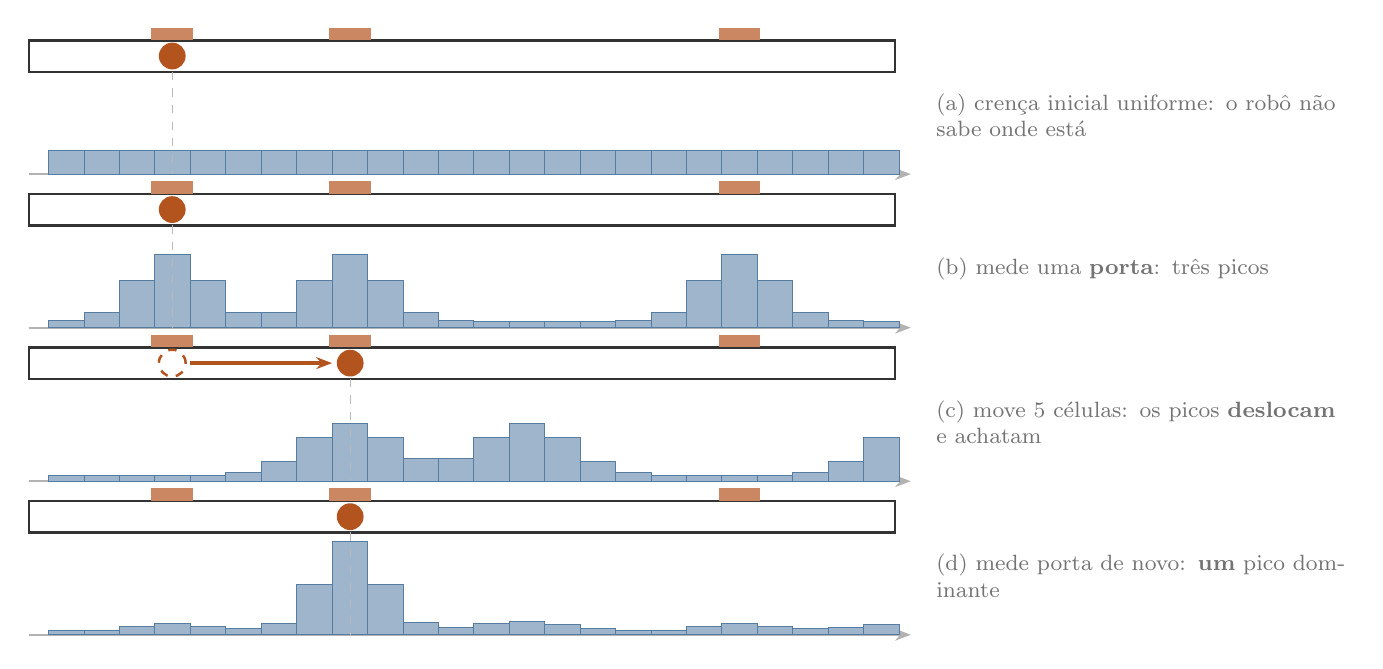
\begin{tikzpicture}[x=1cm,y=1cm]
  \newcommand{\hist}[2]{% y, alturas
    \draw[daxis] (0,#1) -- (11.2,#1);
    \foreach \h [count=\i] in {#2} { \fill[dblue!45, draw=dblue!80, line width=0.3pt] ({0.25+(\i-1)*0.45},#1) rectangle ({0.25+\i*0.45},{#1+\h}); }
  }
  \hist{5.85}{0.30,0.30,0.30,0.30,0.30,0.30,0.30,0.30,0.30,0.30,0.30,0.30,0.30,0.30,0.30,0.30,0.30,0.30,0.30,0.30,0.30,0.30,0.30,0.30}
  \draw[dbody, fill=white, line width=0.9pt] (0,7.15) rectangle (11,7.55);
  \fill[dorange!70] (1.55,7.55) rectangle (2.09,7.71);
  \fill[dorange!70] (3.81,7.55) rectangle (4.35,7.71);
  \fill[dorange!70] (8.76,7.55) rectangle (9.29,7.71);
  \fill[dorange] (1.82,7.35) circle (0.17);
  \draw[dguide] (1.82,7.15) -- (1.82,5.85);
  \node[dlbl, font=\footnotesize, anchor=west, text width=5.2cm] at (11.4,6.60) {(a) crença inicial uniforme: o robô não sabe onde está};
  \hist{3.90}{0.09,0.20,0.60,0.93,0.60,0.20,0.20,0.60,0.93,0.60,0.20,0.09,0.08,0.08,0.08,0.08,0.09,0.20,0.60,0.93,0.60,0.20,0.09,0.08}
  \draw[dbody, fill=white, line width=0.9pt] (0,5.20) rectangle (11,5.60);
  \fill[dorange!70] (1.55,5.60) rectangle (2.09,5.76);
  \fill[dorange!70] (3.81,5.60) rectangle (4.35,5.76);
  \fill[dorange!70] (8.76,5.60) rectangle (9.29,5.76);
  \fill[dorange] (1.82,5.40) circle (0.17);
  \draw[dguide] (1.82,5.20) -- (1.82,3.90);
  \node[dlbl, font=\footnotesize, anchor=west, text width=5.2cm] at (11.4,4.65) {(b) mede uma \textbf{porta}: três picos};
  \hist{1.95}{0.07,0.07,0.07,0.07,0.07,0.11,0.25,0.55,0.73,0.55,0.29,0.29,0.55,0.73,0.55,0.25,0.11,0.07,0.07,0.07,0.07,0.11,0.25,0.55}
  \draw[dbody, fill=white, line width=0.9pt] (0,3.25) rectangle (11,3.65);
  \fill[dorange!70] (1.55,3.65) rectangle (2.09,3.81);
  \fill[dorange!70] (3.81,3.65) rectangle (4.35,3.81);
  \fill[dorange!70] (8.76,3.65) rectangle (9.29,3.81);
  \draw[dorange, dashed, line width=0.9pt, fill=white] (1.82,3.45) circle (0.17);
  \draw[dorange, line width=1.3pt, -{Stealth[length=2mm]}] (2.04,3.45) -- (3.85,3.45);
  \fill[dorange] (4.08,3.45) circle (0.17);
  \draw[dguide] (4.08,3.25) -- (4.08,1.95);
  \node[dlbl, font=\footnotesize, anchor=west, text width=5.2cm] at (11.4,2.70) {(c) move 5 células: os picos \textbf{deslocam} e achatam};
  \hist{0.00}{0.05,0.06,0.11,0.14,0.11,0.08,0.15,0.64,1.18,0.64,0.16,0.09,0.14,0.17,0.13,0.08,0.05,0.06,0.11,0.14,0.11,0.08,0.09,0.13}
  \draw[dbody, fill=white, line width=0.9pt] (0,1.30) rectangle (11,1.70);
  \fill[dorange!70] (1.55,1.70) rectangle (2.09,1.86);
  \fill[dorange!70] (3.81,1.70) rectangle (4.35,1.86);
  \fill[dorange!70] (8.76,1.70) rectangle (9.29,1.86);
  \fill[dorange] (4.08,1.50) circle (0.17);
  \draw[dguide] (4.08,1.30) -- (4.08,0.00);
  \node[dlbl, font=\footnotesize, anchor=west, text width=5.2cm] at (11.4,0.75) {(d) mede porta de novo: \textbf{um} pico dominante};
\end{tikzpicture}
\end{document}
